%%%%%%%%%%%%%%%%%%%%%%%%%%%%%%%%%%%%%%%%%%%%%%%%
%% Compile the master file!
%% 		Include: Antonio Machicao y Priemer
%% 		Course: GK Linguistik
%%%%%%%%%%%%%%%%%%%%%%%%%%%%%%%%%%%%%%%%%%%%%%%%

%\exewidth{(35)} im übergeordneten File

% sollte zentral geladen werden. St. Mü. 04.11.2016 (in localcommands?)
%%%%%%%%%%%%%
%%% Forestset Syllables

\newbox\foreststrutbox
\setbox\foreststrutbox=\hbox to 0pt{\phantom{\forestOve{standard node}{content}}}
\def\foreststrut{\copy\foreststrutbox}
\forestset{
GP1/.style 2 args={
for n={1}{baseline},
s sep=0pt, l sep=0pt,
for descendants={
l sep=0pt, l={#1},
anchor=base,calign=first,child anchor=north,
inner xsep=1pt,inner ysep=2pt,outer sep=0pt,s sep=0pt,
},
delay={
if content={}{phantom}{for children={no edge}},
for tree={
if content={O}{tier=OR}{},
if content={R}{tier=OR}{},
if content={N}{tier=N}{},
if content={x}{
tier=x,content={$\times$},outer xsep={#2},
for tree={calign=center},
for descendants={content format={\foreststrut\forestoption{content}}},
before drawing tree={outer xsep=0pt,delay={typeset node}},
s sep=4pt
}{},
},
},
before drawing tree={where content={}{parent anchor=center,child anchor=center}{}},
},
GP1/.default={5ex}{8.0pt},
associate/.style={%
tikz+={\draw(!)--(!#1);}},
spread/.style={
before drawing tree={tikz+={\draw[dotted](!)--(!#1);}}},
govern/.style={
before drawing tree={tikz+={\draw[->](!)--(!#1);}}},
p-govern/.style={
before drawing tree={tikz+={\draw[->](.north) to[out=150,in=30] (!#1.north);}}},
no p-govern/.style={
before drawing tree={tikz+={\draw[->,loosely dashed](.north) to[out=150,in=30] (!#1.north);}}},
encircle/.style={before drawing tree={circle,draw,inner sep=0pt}},
fen/.style={pin={[font=\footnotesize,inner sep=1pt,pin edge=<-]10:\textsc{Fen}}},
el/.style={content=\textsc{\textbf{##1}}},
head/.style={content=\textsc{\textbf{\underline{##1}}}},
llap/.style={
tikz+={%
\edef\forest@temp{\noexpand\node[\option{node options},
anchor=base east,at=(.base east)]}%
\forest@temp{#1\phantom{\option{environment}}};
}
},
rlap/.style={
tikz+={%
\edef\forest@temp{\noexpand\node[\option{node options},
anchor=base west,at=(.base west)]}%
\forest@temp{\phantom{\option{environment}}#1};
}
},
}
%%%%%%%%%%%%%


%%%%%%%%%%%%%%%%%%%%%%%%%%%%%%%%%%%%%%%%%%%%%%%%%%%%
%%%             Metadata                         
%%%%%%%%%%%%%%%%%%%%%%%%%%%%%%%%%%%%%%%%%%%%%%%%%%%% 

\title{Grundkurs Linguistik}

\subtitle{Phonologie III: Silbenmodelle}

\author[aMyP]{
	{\small Antonio Machicao y Priemer}
	\\
	{\footnotesize \url{http://www.linguistik.hu-berlin.de/staff/amyp}}
	%	\\
	%	{\small\href{mailto:mapriema@hu-berlin.de}{mapriema@hu-berlin.de}}
}

\institute{Institut für deutsche Sprache und Linguistik}

% bitte lassen, sonst kann man nicht sehen, von wann die PDF-Datei ist.
%\date{ }

%\publishers{\textbf{6. linguistischer Methodenworkshop \\ Humboldt-Universität zu Berlin}}

%\hyphenation{nobreak}


%%%%%%%%%%%%%%%%%%%%%%%%%%%%%%%%%%%%%%%%%%%%%%%%%%%%
%%%             Preamble's End                  
%%%%%%%%%%%%%%%%%%%%%%%%%%%%%%%%%%%%%%%%%%%%%%%%%%%%   


%%%%%%%%%%%%%%%%%%%%%%%%%   
\huberlintitlepage[22pt]
\iftoggle{toc}{
\frame{
%\begin{multicols}{2}
	\frametitle{Inhaltsverzeichnis}
	\tableofcontents
	%[pausesections]
%\end{multicols}
}
}

%%%%%%%%%%%%%%%%%%%%%%%%%%%%%%%%%%
%%%%%%%%%%%%%%%%%%%%%%%%%%%%%%%%%%
%%%%%LITERATURE:

%% Allgemein
\nocite{Glueck&Roedel16a}
\nocite{Schierholz&Co18}
\nocite{Luedeling2009a}
\nocite{Meibauer&Co07a} 
\nocite{Repp&Co15a} 

%%% Sprache & Sprachwissenschaft
%\nocite{Fries16c} %Adäquatheit
%\nocite{Fries16a} %Grammatikalität
%\nocite{Fries&MyP16c} %GG
%\nocite{Fries&MyP16b} %Akzeptabilität
%\nocite{Fries&MyP16d} %Kompetenz vs. Performanz

%% Phonetik & Phonologie
\nocite{Altmann&Co07a}
\nocite{DudenAussprache00a}
\nocite{Hall00a} 
\nocite{Kohler99a}
\nocite{Krech&Co09a}
\nocite{Pompino95a}
\nocite{Ramers08a}
\nocite{Ramers&Vater92a}
\nocite{Rues&Co07a}
\nocite{WieseR96a}
\nocite{WieseR11a}


%%%%%%%%%%%%%%%%%%%%%%%%%%%%%%%%%%
%%%%%%%%%%%%%%%%%%%%%%%%%%%%%%%%%%
\section{Phonologie III: Silbenmodelle}
%%%%%%%%%%%%%%%%%%%%%%%%%%%%%%%%%%


%%%%%%%%%%%%%%%%%%%%%%%%%%%%%%%%%%
%%%%%%%%%%%%%%%%%%%%%%%%%%%%%%%%%%
\subsection{Silbenmodelle}

%% MyP: Contents
\iftoggle{sectoc}{
	\frame{
		%\begin{multicols}{2}
		\frametitle{~}
		\tableofcontents[currentsubsection, subsubsectionstyle=hide]
		%\end{multicols}
	}
}

%% StM: Contents
\iftoggle{gliederung}{
	
	\outline{
		\begin{itemize}
			
			\item \blaubf{Silbenmodelle}
			%% CV-Modell
			%% Konstituentenmodell
			\item Silbengelenk
			\item Silbifizierung
			\item Exkurs: Akzent
			\item Hausaufgabe
			
		\end{itemize}
	}
}
%%%%%%%%%%%%%%%%%%%%%%%%%%%%%%%%%%

\begin{frame}
\frametitle{Silbenmodelle}

\begin{itemize}
	\item Bisher (hauptsächlich) nur \textbf{lineare Betrachtung} mit allen Segmenten auf einer Schicht
	\ea
	\textipa{/pe:.t@\textscr /} (Peter)
	\z
	
	\ea
	\textipa{/vE\.t@\textscr /} (Vetter)
	\z
	
	\item \textbf{Nicht-lineare Phonologie} (Autosegmentale Phonologie)
	
	\begin{itemize}
		\item verschiedene Repräsentationsebenen bzw. Schichten
		
		\item hierarchische Strukturierung
		
		\item Vorteil: 
		
		Beschreibung von \textbf{Merkmalsausbreitung} und \textbf{segmentunabhängigen Prozessen}
		
	\end{itemize}
\end{itemize}

\end{frame}


%%%%%%%%%%%%%%%%%%%%%%%%%%%%%%%%%%
%%%%%%%%%%%%%%%%%%%%%%%%%%%%%%%%%%
\subsubsection{CV-Modell}
%\frame{
%\frametitle{~}
%	\tableofcontents[currentsection]
%}
%%%%%%%%%%%%%%%%%%%%%%%%%%%%%%%%%%

\begin{frame}%[shrink]
\frametitle{CV-Modell (einfaches Modell)}

\begin{itemize}
\item Silben und Segmente auf unterschiedlichen Schichten

\item verbunden durch Assoziationslinien

\item Charakterisierung der Silbenstruktur durch C und V 
\end{itemize}

\begin{columns}
	
\column[c]{.45\textwidth}
\begin{figure}
	\centering
	\begin{forest}
		MyP edges,
		[$\sigma$
		[C [\textipa{b}]]
		[C [\textipa{l}]]
		[V [\textipa{I}]]
		[C [\textipa{n}]]
		[C [\textipa{t}]]
		]
	\end{forest}
	\caption{CV-Modell}
\end{figure}


\column[c]{.5\textwidth}
$\sigma :=$ Silbe

C $:=$ nicht-silbisch, \gqq{konsonantisch}

V $:=$ silbisch, \gqq{vokalisch}

\end{columns}

\end{frame}


%%%%%%%%%%%%%%%%%%%%%%%%%%%%%%%%%%
\begin{frame}
\frametitle{Verteilung von Segmenten in der Silbe}

\begin{itemize}
\item Wie ist die Verteilung von Segmenten in der Silbe (im Deutschen)?
\end{itemize}

\begin{minipage}{.59\textwidth}
	\begin{itemize}
	\item C $\neq$ Konsonant, sondern \alertred{nicht-silbisch}
	
	\item V $\neq$ Vokal, sondern \alertblue{silbisch}
	
	\item Jede Silbe enthält \alertgreen{einen Kern} (V).
	\end{itemize}
\end{minipage}
%
\begin{minipage}{.4\textwidth}

\begin{figure}
%\tiny
\small
\centering
\begin{forest}
	MyP edges,
	[$\sigma$
	[C [\textipa{g}]]
	[C [\textipa{l}]]
	[\alertgreen{V} [\textipa{a}]]	
	[C [\alertred{\textipa{U}}]]
	[C [\textipa{p}]]
	[C [\textipa{t}]]
	]
\end{forest}

\begin{forest}
	MyP edges,
	[,phantom
	[$\sigma$
	[C [\textipa{k}]]
	[\alertgreen{V} [\textipa{U}]]
	[C [\textipa{m}]]
	]
	[$\sigma$	
	[C [\textipa{p}]]
	[\alertgreen{V} [\alertblue{\textipa{\textsyllabic{l}}}]]
	]
	]
\end{forest}

\end{figure}

\end{minipage}

% u bei glaubt ist ein C, weil nur a der Silbengipfel ist, u ist weniger sonor, und Diphtonge gelten
% als zwei Zeiteinheiten, bei langen Vokalen wird auch auf zwei geteilt. Der Doppelpunkt ist dann
% ein C

% Bei Beirisch guot geht der Sonoritätsgipfel aufs o und dann ist das o V und davor ein C

\end{frame}


%%%%%%%%%%%%%%%%%%%%%%%%%%%%%%%%%%
\begin{frame}
\frametitle{Verteilung von Segmenten in der Silbe}


\begin{minipage}{.59\textwidth}
	\begin{itemize}
	\item \textbf{maximale Anzahl an Cs} vor und nach V
	
	% Aber strumpfst. Es kommt ein weiteres verbessertes Modell
	
	\item Korrelation zwischen Anzahl an Cs nach V und der \textbf{Länge}/(Un-)Gespanntheit des Vokals
	\end{itemize}
\end{minipage}
%
\begin{minipage}{.4\textwidth}

\begin{figure}
	%\tiny
	\small
	\centering
	\begin{forest}
	MyP edges,
	[$\sigma$
	[C [\textipa{g}]]
	[C [\textipa{l}]]
	[V [\textipa{a}]]	
	[\alertred{C} [\textipa{U}]]
	[\alertred{C} [\textipa{p}]]
	[\alertred{C} [\textipa{t}]]
	]
	\end{forest}
	
	\begin{forest}
	MyP edges,
	[$\sigma$
	[C [\textipa{k}]]
	[C [\textipa{\textscr }]]
	[V [\textipa{a}]]
	[C [\textipa{N}]]
	[C [\textipa{k}]]	
	]
	\end{forest}

\end{figure}

\end{minipage}

% Kopf pf ist ein C
% Kumpel fällt das e weg und wir haben einen vokalischen Konsonant l

\end{frame}



%%%%%%%%%%%%%%%%%%%%%%%%%%%%%%%%%%
\begin{frame}
\frametitle{Verteilung von Segmenten in der Silbe}


\begin{columns}

\column[t]{.49\textwidth}	
	\begin{itemize}
		\item Diphthonge: \textbf{VC} (bzw. CV \textipa{[g\textsubarch{U}Ot]})
	
		\item lange Vokale: \textbf{VC}
	\end{itemize}

\column[t]{.49\textwidth}
	\begin{itemize}
		\item Affrikate: \textbf{C}
	
		\item silbische Konsonanten: \textbf{V}
	\end{itemize}
\end{columns}


\begin{minipage}{.49\textwidth}

	\begin{figure}
%	\tiny
%	\scriptsize
	\small
	\centering
	\begin{forest}
		MyP edges,
		[$\sigma$
		[C [\textipa{g}]]
		[C [\textipa{l}]]
		[V [\alertred{\textipa{a}}]]	
		[C [\alertred{\textipa{U}}]]
		[C [\textipa{p}]]
		[C [\textipa{t}]]
		]
	\end{forest}
	
	\begin{forest}
		MyP edges,
		[$\sigma$
		[C [\textipa{k}]]
		[V [\alertred{\textipa{a}}]]
		[C [\alertred{\textipa{:}}]]	
		[C [\textipa{l}]]
		]
	\end{forest}
	\end{figure}	

\end{minipage}
%
\begin{minipage}{.49\textwidth}

	\begin{figure}
%	\tiny
%	\scriptsize
	\small
	\centering

	\begin{forest}
	MyP edges,
	[$\sigma$
	[C [\textipa{k}]]
	[V [\textipa{O}]]
	[C [\alertred{\textipa{\t{pf}}}]]	
	[C [\textipa{s}]]
	]
	\end{forest}
	
	\begin{forest}
	MyP edges,
	[,phantom
	[$\sigma$
	[C [\textipa{k}]]
	[V [\textipa{U}]]
	[C [\textipa{m}]]	
	]
	[$\sigma$
	[C [\textipa{p}]]
	[V [\alertred{\textipa{\textsyllabic{l}}}]]
	]
	]
	\end{forest}

\end{figure}

\end{minipage}

\end{frame}



%%%%%%%%%%%%%%%%%%%%%%%%%%%%%%%%%%
%%%%%%%%%%%%%%%%%%%%%%%%%%%%%%%%%%
\subsubsection{Konstituentenmodell}
%\frame{
%\begin{multicols}{2}
%\frametitle{~}
%	\tableofcontents[currentsection]
%\end{multicols}
%}
%%%%%%%%%%%%%%%%%%%%%%%%%%%%%%%%%%

\begin{frame}
\frametitle{Konstituentenmodell}

\begin{itemize}
\item Zerlegung in \textbf{silbische Konstituenten}
\item Silbe ($\sigma$) $=$ Onset (O) $+$ Reim (R)
\item Reim (R) $=$ Nukleus (N) $+$ Koda (K)
\item $+$ Skelettschicht (X)
\end{itemize}

% nur x, C und V braucht man nicht mehr, weil N das V (vokalische Element) ist
% x sind die Zeiteinheiten

\begin{figure}
%%%%%%%%%%%%%%
%%% Forestset Syllables

\newbox\foreststrutbox
\setbox\foreststrutbox=\hbox to 0pt{\phantom{\forestOve{standard node}{content}}}
\def\foreststrut{\copy\foreststrutbox}
\forestset{
GP1/.style 2 args={
for n={1}{baseline},
s sep=0pt, l sep=0pt,
for descendants={
l sep=0pt, l={#1},
anchor=base,calign=first,child anchor=north,
inner xsep=1pt,inner ysep=2pt,outer sep=0pt,s sep=0pt,
},
delay={
if content={}{phantom}{for children={no edge}},
for tree={
if content={O}{tier=OR}{},
if content={R}{tier=OR}{},
if content={N}{tier=N}{},
if content={x}{
tier=x,content={$\times$},outer xsep={#2},
for tree={calign=center},
for descendants={content format={\foreststrut\forestoption{content}}},
before drawing tree={outer xsep=0pt,delay={typeset node}},
s sep=4pt
}{},
},
},
before drawing tree={where content={}{parent anchor=center,child anchor=center}{}},
},
GP1/.default={5ex}{8.0pt},
associate/.style={%
tikz+={\draw(!)--(!#1);}},
spread/.style={
before drawing tree={tikz+={\draw[dotted](!)--(!#1);}}},
govern/.style={
before drawing tree={tikz+={\draw[->](!)--(!#1);}}},
p-govern/.style={
before drawing tree={tikz+={\draw[->](.north) to[out=150,in=30] (!#1.north);}}},
no p-govern/.style={
before drawing tree={tikz+={\draw[->,loosely dashed](.north) to[out=150,in=30] (!#1.north);}}},
encircle/.style={before drawing tree={circle,draw,inner sep=0pt}},
fen/.style={pin={[font=\footnotesize,inner sep=1pt,pin edge=<-]10:\textsc{Fen}}},
el/.style={content=\textsc{\textbf{##1}}},
head/.style={content=\textsc{\textbf{\underline{##1}}}},
llap/.style={
tikz+={%
\edef\forest@temp{\noexpand\node[\option{node options},
anchor=base east,at=(.base east)]}%
\forest@temp{#1\phantom{\option{environment}}};
}
},
rlap/.style={
tikz+={%
\edef\forest@temp{\noexpand\node[\option{node options},
anchor=base west,at=(.base west)]}%
\forest@temp{\phantom{\option{environment}}#1};
}
},
}
%%%%%%%%%%%%%

\centering
\scalebox{.8}{
\begin{forest} MyP edges, [,phantom
[$\sigma$
[O[x, tier=word[\textipa{f}]][x, tier=word[\textipa{K}]]]
[R[N[x, tier=word[\textipa{\textopeno}]]][K[x[\textipa{s}]]]]
]
[$\sigma$
[O[x, tier=word[\textipa{t}]]]
[R[N[x[\textipa{I}]]][K[x[\c{c}]]]]
]  
]
\end{forest}}

% frostig
%\caption{Konstituentenmodell}
\end{figure}

\end{frame}



%%%%%%%%%%%%%%%%%%%%%%%%%%%%%%%%%%

\begin{frame}
\frametitle{Silbe, Onset und Reim}

\textbf{Silbe} ($\sigma$) = Onset (O) + Reim (R)

\begin{itemize}
\item \textbf{Onset}: 

	\begin{itemize}
		\item Evidenz aus Versprecherforschung
		
		\ea
		\textipa{\alertred{k}Il\c{c}.\alertblue{m}a\.fe:} vs. \textipa{\alertblue{m}Il\c{c}.\alertred{k}a\.fe:} (nicht \textipa{k\textbf{a}l\c{c}.m\textbf{I}\.fe:})
		\z
		% Versprecher: Kilchmafee für   Milchkafee
		% Aber keinen Versprecher * Kalchmifee
	\end{itemize}	

\pause 

\item \textbf{Reim}: 
	\begin{itemize}
		\item Silbengewicht: Längenausgleich zwischen N und K 		
		% Onset ist für den Längenausgleich irrelevant. wenn Koda lang, dann Nukleus kurz. Findet alles
		% innerhalb des Reims statt
		
		% Auch Auslautverhärtung findet in der Koda statt:
		% sagst -> sakst, d.h. g ist in der Koda
		
		\item Gedichte
		\item typischerweise VCC (auch als VVC kodiert)
	\end{itemize}

\end{itemize}

\textbf{Reim} (R) = Nukleus (N) + Koda (K)

	\begin{itemize}
		\item \textbf{Nukleus}: obligatorischer Bestandteil der Silbe
		
		\item \textbf{Koda}: Regeln, die sich nur auf die Konsonanten in der Koda beziehen
	\end{itemize}

\end{frame}


%%%%%%%%%%%%%%%%%%%%%%%%%%%%%%%%%
\begin{frame}[shrink]
\frametitle{Skelettschicht}

\begin{itemize}
\item Ebene zwischen den Segmenten und den Silbenkonstituenten

\item X $:=$ abstrakte Zeiteinheit (\zB für Darstellung des Längenausgleichs)

\item X \ras vergleichbar mit C und V

\item \textbf{Nukleus}:

\begin{itemize}
\item 1 X: Kurzvokal, silbischer Konsonant
\item 2 X: Langvokal, Diphthong
\item (3 X: Langvokal + vokalisiertes \textipa{/\textscr /} -- umstritten)
\end{itemize}

\end{itemize}


\begin{minipage}{.325\textwidth}

%%%%%%%%%%%%%%
%%% Forestset Syllables

\newbox\foreststrutbox
\setbox\foreststrutbox=\hbox to 0pt{\phantom{\forestOve{standard node}{content}}}
\def\foreststrut{\copy\foreststrutbox}
\forestset{
GP1/.style 2 args={
for n={1}{baseline},
s sep=0pt, l sep=0pt,
for descendants={
l sep=0pt, l={#1},
anchor=base,calign=first,child anchor=north,
inner xsep=1pt,inner ysep=2pt,outer sep=0pt,s sep=0pt,
},
delay={
if content={}{phantom}{for children={no edge}},
for tree={
if content={O}{tier=OR}{},
if content={R}{tier=OR}{},
if content={N}{tier=N}{},
if content={x}{
tier=x,content={$\times$},outer xsep={#2},
for tree={calign=center},
for descendants={content format={\foreststrut\forestoption{content}}},
before drawing tree={outer xsep=0pt,delay={typeset node}},
s sep=4pt
}{},
},
},
before drawing tree={where content={}{parent anchor=center,child anchor=center}{}},
},
GP1/.default={5ex}{8.0pt},
associate/.style={%
tikz+={\draw(!)--(!#1);}},
spread/.style={
before drawing tree={tikz+={\draw[dotted](!)--(!#1);}}},
govern/.style={
before drawing tree={tikz+={\draw[->](!)--(!#1);}}},
p-govern/.style={
before drawing tree={tikz+={\draw[->](.north) to[out=150,in=30] (!#1.north);}}},
no p-govern/.style={
before drawing tree={tikz+={\draw[->,loosely dashed](.north) to[out=150,in=30] (!#1.north);}}},
encircle/.style={before drawing tree={circle,draw,inner sep=0pt}},
fen/.style={pin={[font=\footnotesize,inner sep=1pt,pin edge=<-]10:\textsc{Fen}}},
el/.style={content=\textsc{\textbf{##1}}},
head/.style={content=\textsc{\textbf{\underline{##1}}}},
llap/.style={
tikz+={%
\edef\forest@temp{\noexpand\node[\option{node options},
anchor=base east,at=(.base east)]}%
\forest@temp{#1\phantom{\option{environment}}};
}
},
rlap/.style={
tikz+={%
\edef\forest@temp{\noexpand\node[\option{node options},
anchor=base west,at=(.base west)]}%
\forest@temp{\phantom{\option{environment}}#1};
}
},
}
%%%%%%%%%%%%%

\centering
\scalebox{.65}{
\begin{forest} MyP edges, [,phantom 
[$\sigma$
[O
[x, tier=word[\textipa{m}]]
]
[R
[N
[x[\textipa{I}]]
]
[K[x, tier=word[t]]
]
]
]]
\end{forest}}

\end{minipage}
%
\begin{minipage}{.325\textwidth}
%%%%%%%%%%%%%%
%%% Forestset Syllables

\newbox\foreststrutbox
\setbox\foreststrutbox=\hbox to 0pt{\phantom{\forestOve{standard node}{content}}}
\def\foreststrut{\copy\foreststrutbox}
\forestset{
GP1/.style 2 args={
for n={1}{baseline},
s sep=0pt, l sep=0pt,
for descendants={
l sep=0pt, l={#1},
anchor=base,calign=first,child anchor=north,
inner xsep=1pt,inner ysep=2pt,outer sep=0pt,s sep=0pt,
},
delay={
if content={}{phantom}{for children={no edge}},
for tree={
if content={O}{tier=OR}{},
if content={R}{tier=OR}{},
if content={N}{tier=N}{},
if content={x}{
tier=x,content={$\times$},outer xsep={#2},
for tree={calign=center},
for descendants={content format={\foreststrut\forestoption{content}}},
before drawing tree={outer xsep=0pt,delay={typeset node}},
s sep=4pt
}{},
},
},
before drawing tree={where content={}{parent anchor=center,child anchor=center}{}},
},
GP1/.default={5ex}{8.0pt},
associate/.style={%
tikz+={\draw(!)--(!#1);}},
spread/.style={
before drawing tree={tikz+={\draw[dotted](!)--(!#1);}}},
govern/.style={
before drawing tree={tikz+={\draw[->](!)--(!#1);}}},
p-govern/.style={
before drawing tree={tikz+={\draw[->](.north) to[out=150,in=30] (!#1.north);}}},
no p-govern/.style={
before drawing tree={tikz+={\draw[->,loosely dashed](.north) to[out=150,in=30] (!#1.north);}}},
encircle/.style={before drawing tree={circle,draw,inner sep=0pt}},
fen/.style={pin={[font=\footnotesize,inner sep=1pt,pin edge=<-]10:\textsc{Fen}}},
el/.style={content=\textsc{\textbf{##1}}},
head/.style={content=\textsc{\textbf{\underline{##1}}}},
llap/.style={
tikz+={%
\edef\forest@temp{\noexpand\node[\option{node options},
anchor=base east,at=(.base east)]}%
\forest@temp{#1\phantom{\option{environment}}};
}
},
rlap/.style={
tikz+={%
\edef\forest@temp{\noexpand\node[\option{node options},
anchor=base west,at=(.base west)]}%
\forest@temp{\phantom{\option{environment}}#1};
}
},
}
%%%%%%%%%%%%%

\centering
\scalebox{.65}{
\begin{forest} MyP edges, [,phantom
[$\sigma$
[O[x, tier=word[\textipa{z}]]]
[R
[N
[x, tier=word
[\textipa{e:}, name=e]
]
[x, name=x]
] ]
] ]
{
\draw[black] (e.north)--(x.south);
}
\end{forest}}

\end{minipage}
%
\begin{minipage}{.325\textwidth}
%%%%%%%%%%%%%%
%%% Forestset Syllables

\newbox\foreststrutbox
\setbox\foreststrutbox=\hbox to 0pt{\phantom{\forestOve{standard node}{content}}}
\def\foreststrut{\copy\foreststrutbox}
\forestset{
GP1/.style 2 args={
for n={1}{baseline},
s sep=0pt, l sep=0pt,
for descendants={
l sep=0pt, l={#1},
anchor=base,calign=first,child anchor=north,
inner xsep=1pt,inner ysep=2pt,outer sep=0pt,s sep=0pt,
},
delay={
if content={}{phantom}{for children={no edge}},
for tree={
if content={O}{tier=OR}{},
if content={R}{tier=OR}{},
if content={N}{tier=N}{},
if content={x}{
tier=x,content={$\times$},outer xsep={#2},
for tree={calign=center},
for descendants={content format={\foreststrut\forestoption{content}}},
before drawing tree={outer xsep=0pt,delay={typeset node}},
s sep=4pt
}{},
},
},
before drawing tree={where content={}{parent anchor=center,child anchor=center}{}},
},
GP1/.default={5ex}{8.0pt},
associate/.style={%
tikz+={\draw(!)--(!#1);}},
spread/.style={
before drawing tree={tikz+={\draw[dotted](!)--(!#1);}}},
govern/.style={
before drawing tree={tikz+={\draw[->](!)--(!#1);}}},
p-govern/.style={
before drawing tree={tikz+={\draw[->](.north) to[out=150,in=30] (!#1.north);}}},
no p-govern/.style={
before drawing tree={tikz+={\draw[->,loosely dashed](.north) to[out=150,in=30] (!#1.north);}}},
encircle/.style={before drawing tree={circle,draw,inner sep=0pt}},
fen/.style={pin={[font=\footnotesize,inner sep=1pt,pin edge=<-]10:\textsc{Fen}}},
el/.style={content=\textsc{\textbf{##1}}},
head/.style={content=\textsc{\textbf{\underline{##1}}}},
llap/.style={
tikz+={%
\edef\forest@temp{\noexpand\node[\option{node options},
anchor=base east,at=(.base east)]}%
\forest@temp{#1\phantom{\option{environment}}};
}
},
rlap/.style={
tikz+={%
\edef\forest@temp{\noexpand\node[\option{node options},
anchor=base west,at=(.base west)]}%
\forest@temp{\phantom{\option{environment}}#1};
}
},
}
%%%%%%%%%%%%%

\centering
\scalebox{.65}{\begin{forest} MyP edges, [,phantom 
[$\sigma$
[O[x, tier=word[\textipa{P}]]]
[R
[N
[x, tier=word
[\textipa{\t{aU}}, name=aU]
]
[x, name=x]
]
[K[x[\textipa{x}]]]]
] ]
{
\draw[black] (aU.north)--(x.south);
}
\end{forest}}

\end{minipage}

% Bei bar kann nach dem langen a das r noch zum Nukleus gerechnet werden, als drittes x. Oder in
% eben in der Koda.

\end{frame}



%%%%%%%%%%%%%%%%%%%%%%%%%%%%%%%%%

\begin{frame}
\frametitle{Skelettschicht}

\begin{itemize}

\item \textbf{Onset} und \textbf{Koda}:

\begin{itemize}
\item pro C ein X
\item<2-> Achtung: \alertred{Affrikate} \ras 1 X (eine Zeiteinheit!)
\item<3-> Ausnahme: \alertblue{Silbengelenk} (s.u.)

\end{itemize}
\end{itemize}

\hfill
\footnotesize
\visible<1->{
\begin{forest} MyP edges, [,phantom
[$\sigma$
[O
[x, tier=word[\textipa{f}]]
[x, tier=word[\textipa{\textscr }]]
]
[R
[N
[x, tier=word
[\textipa{E}]
]
]
[K [x[\textipa{\c{c}}]]]]
]  
]
\end{forest}
}
\hfill
\visible<2->{%
\begin{forest} MyP edges, [,phantom
[$\sigma$
[O
[x, tier=word[\textipa{k}]]
]
[R
[N
[x, tier=word[\textipa{O}]]
]
[K
[\alertred{x}[\alertred{\textipa{\t{pf}}}]]
]
]
]]
\end{forest}}
\hfill
\visible<3->{\begin{forest} MyP edges, [,phantom
[$\sigma$
[O
[x, tier=word
[\textipa{m}]
]
]
[R
[N
[x, tier=word
[\textipa{I}]
]
]  		
[K 
[\alertblue{x}, name=x
[\alertblue{\textipa{t}}]
]
]
]
]
[$\sigma$
[O, name=O
]
[R
[N
[x
[\textipa{@}]
]
]
[K [x[\textipa{n}]]]]
]  
]
{
\draw[black] (x.north)--(O.south);
}
\end{forest}}
\hfill\mbox{}

\end{frame}


%%%%%%%%%%%%%%%%%%%%%%%%%%%%%%%%%%%
\begin{frame}
\frametitle{Reim: Vokallänge und Besetzung der Koda}

%Zusammenhang zwischen Vokallänge und Besetzung der Koda \ras Reim

\begin{columns}

\column[t]{.5\textwidth}	
\begin{block}{Lange Vokale}
Nach einem langen Vokal oder einem Diphthong steht in monomorphemischen Silben \textbf{kein Konsonantencluster}. 

Es gibt wenige Ausnahmen: \emph{Mo\textbf{nd}}, \emph{O\textbf{bst}}.
\end{block}


\column[t]{.5\textwidth}
\begin{block}{Kurze Vokale}
In betonten Silben folgt auf ungespannten (kurzen) Vokal \textbf{meistens ein Konsonant}.\par
Ausnahmen in Fremdwörtern: \emph{\textbf{a}.sozial}
\end{block}	

\end{columns}


\begin{minipage}{.325\textwidth}
	\footnotesize
	\centering
	\begin{forest} MyP edges, [,phantom
	[$\sigma$
	[O[x, tier=word[\textipa{z}]]]
	[R
	[N
	[x, tier=word
	[\textipa{e:}, name=e]
	]
	[x, name=x]
	]
	]
	]  
	]
	{
	\draw[black] (e.north)--(x.south);
	}
	\end{forest}
\end{minipage}
%
\begin{minipage}{.325\textwidth}
	\footnotesize
	\centering
	\begin{forest} MyP edges, [,phantom
	[$\sigma$
	[O[x, tier=word[\textipa{P}]]]
	[R
	[N
	[x, tier=word
	[\textipa{\t{aU}}, name=aU]
	]
	[x, name=x]
	]
	[K[x[\textipa{x}]]]]
	]  
	]
	{
	\draw[black] (aU.north)--(x.south);
	}
	\end{forest}
\end{minipage}
%
\begin{minipage}{.325\textwidth}
	\footnotesize
	\centering
	\begin{forest} MyP edges, [,phantom
	[$\sigma$
	[O
	[x, tier=word[\textipa{m}]]
	]
	[R
	[N
	[x, tier=word[\textipa{I}]]]
	[K
	[x[t]]
	]
	]
	]]
	\end{forest}
\end{minipage}

\end{frame}


%%%%%%%%%%%%%%%%%%%%%%%%%%%%%%%%%%%
%%%%%%%%%%%%%%%%%%%%%%%%%%%%%%%%%%%
\subsection{Silbengelenk}

%% MyP: Contents
\iftoggle{sectoc}{
	\frame{
		%\begin{multicols}{2}
		\frametitle{~}
		\tableofcontents[currentsubsection, subsubsectionstyle=hide]
		%\end{multicols}
	}
}

%% StM: Contents
\iftoggle{gliederung}{
	
	\outline{
		\begin{itemize}
			
			\item Silbenmodelle
			%% CV-Modell
			%% Konstituentenmodell
			\item \blaubf{Silbengelenk}
			\item Silbifizierung
			\item Exkurs: Akzent
			\item Hausaufgabe
			
		\end{itemize}
	}
}
%%%%%%%%%%%%%%%%%%%%%%%%%%%%%%%%%%

\begin{frame}
\frametitle{Silbengelenk}

\begin{minipage}{.63\textwidth}

\begin{itemize}
	\item \textbf{ambisyllabischer Konsonant}
	
	\item[]
	\item Ein Konsonant,\\
	der zugleich \textbf{zu zwei Silben} gehört. 
	
	\item[]
	\item Nur \textbf{eine X Position} (nur eine Zeiteinheit, vgl. echte Geminaten)

\end{itemize}
\end{minipage}
%
\begin{minipage}{.35\textwidth}
	\footnotesize
	\centering
	\begin{forest} MyP edges, [,phantom
	[$\sigma$
	[O
	[x, tier=word
	[\textipa{t}]
	]
	]
	[R
	[N
	[x, tier=word
	[\textipa{I}]
	]
	]  		
	[\alertred{K} 
	[\alertred{x}, name=x
	[\alertred{\textipa{k}}]
	]
	]
	]
	]
	[$\sigma$
	[\alertred{O}, name=onset 
	]
	[R
	[N
	[x
	[\textipa{@}]
	]
	]
	[K [x[\textipa{n}]]]]
	]  
	]
	{
	\draw[black] (x.north)--(onset.south);
	}
	\end{forest}
\end{minipage}

\end{frame}


%%%%%%%%%%%%%%%%%%%%%%%%%%%%%%%%%%
\begin{frame}
\frametitle{Silbengelenk}

\begin{minipage}{.35\textwidth}
	\footnotesize
	\centering
	\begin{forest} MyP edges, [, phantom
	[$\sigma$
	[O
	[x, tier=word
	[\textipa{k}]
	]
	[x, tier=word	[\textipa{l}]]
	]
	[R
	[N
	[x, tier=word
	[\textipa{I}]
	]
	]  		
	[K 
	[x, name=x
	[\textipa{N}]
	]
	]
	]
	]
	[$\sigma$
	[O, name=onset
	]
	[R
	[N
	[x
	[\textipa{@}]
	]
	]
	[K [x[\textipa{n}]]]]
	]  
	]
	{
	\draw[black] (x.north)--(onset.south);
	}
	\end{forest}
\end{minipage}
%
\begin{minipage}{.63\textwidth}

\begin{itemize}
	\item \textbf{In der Schreibung} werden Silbengelenke häufig mit \textbf{Doppelkonsonanten} markiert (aber nicht immer!)
	
	\ea der \textipa{[\t{tS}Et]} \vs ich \textipa{[\t{tS}Et@]}\\
	\pause der Cha\alertred{t} \vs ich cha\alertred{tt}e
	\z
	\ea
	abkli\alertred{ng}en, zwi\alertred{sch}en
	\z
	% abklingngen, zwischschen durch ästhetisches Prinzip verboten
	
	\pause
	
	\item Silbengelenke kommen \textbf{nach betonten ungespannten Vokalen} vor.
	
	Ungespannte betonte Vokale kommen nicht in offenen Silben vor.
	
	\item Linear: \textbf{Markierung} durch Punkt
	
	\ea
	\textipa{[Pap.klI\alertred{\.N}@n]}
	\z

\end{itemize}

\end{minipage}

\end{frame}


%%%%%%%%%%%%%%%%%%%%%%%%%%%%%%%%%%
%%%%%%%%%%%%%%%%%%%%%%%%%%%%%%%%%%

\iftoggle{uebung}{

%\subsection{Übung}
%
%%% MyP: Contents
%\iftoggle{sectoc}{
%	\frame{
%		%\begin{multicols}{2}
%		\frametitle{~}
%		\tableofcontents[currentsubsection, subsubsectionstyle=hide]
%		%\end{multicols}
%	}
%}


%%%%%%%%%%%%%%%%%%%%%%%%%%%%%%%%%%
\begin{frame}
\frametitle{Übung}

Geben Sie eine \textbf{phonetische Transkription} der folgenden Wörter nach der \gqq{Standardaussprache} an, zeichnen Sie dabei die \textbf{Silbenstruktur} nach dem Konstituentenmodell und mit der \textbf{Skelettschicht} und geben Sie die \textbf{Sonoritätsprofile} an.

\begin{block}{Sonoritätshierarchie (Zur Erinnerung)}
Vokal $>$ \textipa{/\textscr /} $>$ \textipa{/l/} $>$ Nasal $>$ Frikativ $>$ Plosiv \\
$x > y :=$ $x$ ist sonorer als $y$
\end{block}

\begin{multicols}{2}
\eal 
\ex sprechen
\ex Obst
\ex Brandschutz
%\ex Stimmenfang
\ex Abstandshalter
%\ex Mittagessen
%\ex Bierdeckel
\zl
\end{multicols}

\end{frame}


} 
%% END true = Q
%% BEGIN false = Q + A
{
%%%%%%%%%%%%%%%%%%%%%%%%%%%%%%%%%%
\begin{frame}
\frametitle{Übung}

Geben Sie eine \textbf{phonetische Transkription} der folgenden Wörter nach der \gqq{Standardaussprache} an, zeichnen Sie dabei die \textbf{Silbenstruktur} nach dem Konstituentenmodell und mit der \textbf{Skelettschicht} und geben Sie die \textbf{Sonoritätsprofile} an.

\begin{block}{Sonoritätshierarchie (Zur Erinnerung)}
	Vokal $>$ \textipa{/\textscr /} $>$ \textipa{/l/} $>$ Nasal $>$ Frikativ $>$ Plosiv \\
	$x > y :=$ $x$ ist sonorer als $y$
\end{block}

\begin{multicols}{2}
	\eal 
	\ex sprechen
	\ex Obst
	\ex Brandschutz
	%\ex Stimmenfang
	\ex Abstandshalter
	%\ex Mittagessen
	%\ex Bierdeckel
	\zl
\end{multicols}

\end{frame}

	
%%%%%%%%%%%%%%%%%%%%%%%%%%%%%%%%%%
\begin{frame}
\frametitle{Lösungen}

\begin{minipage}{.45\textwidth}
\centering
\scalebox{.75}{\begin{forest} MyP edges, [,phantom
[$\sigma$
[O	[x, tier=word [\textipa{S}]
]
[x, tier=word [\textipa{p}]
]
[x, tier=word[\textipa{\textscr}]
]
]
[R
[N	[x, tier=word [\textipa{E}]
]
]
[K, name=K	[x,name=x  [\textipa{\c{c}}]
]
]
]  
]
[$\sigma$
[O, name=O]
[R
[N	[x[\textipa{@}]
]
]
[K	[x[\textipa{n}]
]
]
]
]
]
\draw[black] (O.south)--(x.north);
\end{forest}}
\end{minipage}
\pause
%
\begin{minipage}{.05\textwidth}
\hfill
\end{minipage}
%
\begin{minipage}{.45\textwidth}
%%%%%%%%%%%%%%%
%%% Forestset Syllables

\newbox\foreststrutbox
\setbox\foreststrutbox=\hbox to 0pt{\phantom{\forestOve{standard node}{content}}}
\def\foreststrut{\copy\foreststrutbox}
\forestset{
GP1/.style 2 args={
for n={1}{baseline},
s sep=0pt, l sep=0pt,
for descendants={
l sep=0pt, l={#1},
anchor=base,calign=first,child anchor=north,
inner xsep=1pt,inner ysep=2pt,outer sep=0pt,s sep=0pt,
},
delay={
if content={}{phantom}{for children={no edge}},
for tree={
if content={O}{tier=OR}{},
if content={R}{tier=OR}{},
if content={N}{tier=N}{},
if content={x}{
tier=x,content={$\times$},outer xsep={#2},
for tree={calign=center},
for descendants={content format={\foreststrut\forestoption{content}}},
before drawing tree={outer xsep=0pt,delay={typeset node}},
s sep=4pt
}{},
},
},
before drawing tree={where content={}{parent anchor=center,child anchor=center}{}},
},
GP1/.default={5ex}{8.0pt},
associate/.style={%
tikz+={\draw(!)--(!#1);}},
spread/.style={
before drawing tree={tikz+={\draw[dotted](!)--(!#1);}}},
govern/.style={
before drawing tree={tikz+={\draw[->](!)--(!#1);}}},
p-govern/.style={
before drawing tree={tikz+={\draw[->](.north) to[out=150,in=30] (!#1.north);}}},
no p-govern/.style={
before drawing tree={tikz+={\draw[->,loosely dashed](.north) to[out=150,in=30] (!#1.north);}}},
encircle/.style={before drawing tree={circle,draw,inner sep=0pt}},
fen/.style={pin={[font=\footnotesize,inner sep=1pt,pin edge=<-]10:\textsc{Fen}}},
el/.style={content=\textsc{\textbf{##1}}},
head/.style={content=\textsc{\textbf{\underline{##1}}}},
llap/.style={
tikz+={%
\edef\forest@temp{\noexpand\node[\option{node options},
anchor=base east,at=(.base east)]}%
\forest@temp{#1\phantom{\option{environment}}};
}
},
rlap/.style={
tikz+={%
\edef\forest@temp{\noexpand\node[\option{node options},
anchor=base west,at=(.base west)]}%
\forest@temp{\phantom{\option{environment}}#1};
}
},
}
%%%%%%%%%%%%%

\centering
%\visible<3->
{\scalebox{.75}{\begin{forest} MyP edges, [,phantom
[$\sigma$
[O	[x, tier=word[\textipa{P}]
]
]
[R
[N
[x, tier=word[\textipa{o:}, name=o]
]
[x, name=x]
%    		{\draw[black] (.south)--++(-2.38em,-1.7ex);}
]
[K
[x[\textipa{p}]
]
[x[\textipa{s}]
]
[x[\textipa{t}]
]
]
]  
] ]
\draw[black](x.south)--(o.north);
\end{forest}}}
\end{minipage}
\pause
\begin{minipage}{.45\textwidth}
\begin{figure}
\centering
%		\visible<2->
{\scalebox{.75}{
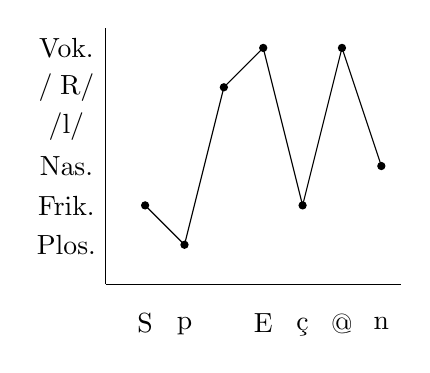
\begin{tikzpicture}[scale=0.5]
\draw[black] (-1,0) -- (6.5,0) ; % x axis
\draw[black] (-1,0) -- (-1,6.5); % y axis
\node at (-2,1) {Plos.};
\node at (-2,2) {Frik.};
\node at (-2,3) {Nas.};
\node at (-2,4) {\textipa{/l/}};
\node at (-2,5) {\textipa{/\;R/}};
\node at (-2,6) {Vok.};
\draw[black] (0,2) -- (1,1) -- (2,5) -- (3,6) -- (4,2) -- (5,6) -- (6,3);
\node at (0,-1) {\textipa{S}};
\node at (1,-1.08) {\textipa{p}};
\node at (2,-1) {\textipa{\textscr}};
\node at (3,-1) {\textipa{E}};
\node at (4,-1.08) {\textipa{\c{c}}};
\node at (5,-1) {\textipa{@}};
\node at (6,-1) {\textipa{n}};
\fill (0,2) circle [radius=3pt];
\fill (1,1) circle [radius=3pt];
\fill (2,5) circle [radius=3pt];
\fill (3,6) circle [radius=3pt];
\fill (4,2) circle [radius=3pt];
\fill (5,6) circle [radius=3pt];
\fill (6,3) circle [radius=3pt];
\end{tikzpicture}}}
\end{figure}
\end{minipage}
\pause
\begin{minipage}{.05\textwidth}
\hfill
\end{minipage}
\begin{minipage}{.45\textwidth}
\begin{figure}
\centering
%\visible<4->
{\scalebox{.75}{
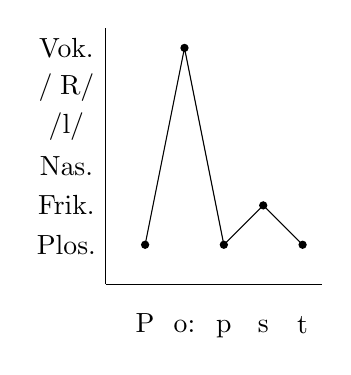
\begin{tikzpicture}[scale=0.5]
\draw[black] (-1,0) -- (4.5,0) ; % x axis
\draw[black] (-1,0) -- (-1,6.5); % y axis
\node at (-2,1) {Plos.};
\node at (-2,2) {Frik.};
\node at (-2,3) {Nas.};
\node at (-2,4) {\textipa{/l/}};
\node at (-2,5) {\textipa{/\;R/}};
\node at (-2,6) {Vok.};
\draw[black] (0,1) -- (1,6) -- (2,1) -- (3,2) -- (4,1);
\node at (0,-1) {\textipa{P}};
\node at (1,-1.08) {\textipa{o:}};
\node at (2,-1.15) {\textipa{p}};
\node at (3,-1.08) {\textipa{s}};
\node at (4,-1.03) {\textipa{t}};
\fill (0,1) circle [radius=3pt];
\fill (1,6) circle [radius=3pt];
\fill (2,1) circle [radius=3pt];
\fill (3,2) circle [radius=3pt];
\fill (4,1) circle [radius=3pt];
\end{tikzpicture}}}
\end{figure}
\end{minipage}

\end{frame}
%%%%%%%%%%%%%%%%%%%%%%%%%%%%%%%%%

\begin{frame}
\frametitle{Lösungen}
%
\begin{minipage}{.3\textwidth}
\centering
\scalebox{.75}{\begin{forest} MyP edges, [,phantom
[$\sigma$
[O
[x, tier=word[\textipa{b}]]
[x, tier=word[\textipa{\textscr}]]
]
[R
[N	[x, tier=word[\textipa{a}]]
]
[K
[x[\textipa{n}]]
[x[\textipa{t}]]
]
]  
]
[$\sigma$
[O	[x, tier=word[\textipa{S}]]
]
[R	
[N	
[x[\textipa{U}]]
]
[K	
[x[\textipa{\t{ts}}]]
]
]
]]
\end{forest}}

\end{minipage}
\pause
%
\begin{minipage}{.05\textwidth}
\hfill
\end{minipage}
%
\begin{minipage}{.6\textwidth}
\centering
\scalebox{.75}{
\begin{forest}
MyP edges, [, phantom
[$ \sigma $
[O
[x, tier=word[\textipa{P}]]
]
[R
[N
[x, tier=word[\textipa{a}]]
]
[K
[x[\textipa{p}]]
]
]
]
[$ \sigma $
[O
[x, tier=word[\textipa{S}]]
[x, tier=word[\textipa{t}]]
]
[R
[N
[x[\textipa{a}]]
]
[K
[x[\textipa{n}]]
[x[\textipa{\t{ts}}]]
]
]
]
[$ \sigma $
[O
[x, tier=word[\textipa{h}]]
]
[R
[N
[x[\textipa{a}]]
]
[K
[x[\textipa{l}]]
]
]
]
[$ \sigma $
[O
[x, tier=word[t]]
]
[R	
[N
[x[\textipa{\textturna}]]
]
]
]]
\end{forest}}
\end{minipage}
\pause
\begin{minipage}{.3\textwidth}
\begin{figure}
\centering
\scalebox{.75}{
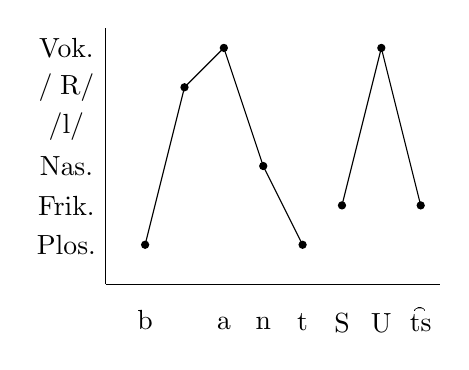
\begin{tikzpicture}[scale=0.5]
\draw[black] (-1,0) -- (7.5,0) ; % x axis
\draw[black] (-1,0) -- (-1,6.5); % y axis
\node at (-2,1) {Plos.};
\node at (-2,2) {Frik.};
\node at (-2,3) {Nas.};
\node at (-2,4) {\textipa{/l/}};
\node at (-2,5) {\textipa{/\;R/}};
\node at (-2,6) {Vok.};
\draw[black] (0,1) -- (1,5) -- (2,6) -- (3,3) -- (4,1);
\draw[black] (5,2) -- (6,6) -- (7,2);
\node at (0,-0.9) {\textipa{b}};
\node at (1,-1) {\textipa{\textscr}};
\node at (2,-1) {\textipa{a}};
\node at (3,-1) {\textipa{n}};
\node at (4,-0.95) {\textipa{t}};
\node at (5,-1) {\textipa{S}};
\node at (6,-1) {\textipa{U}};
\node at (7,-0.9) {\textipa{\t{ts}}};
\fill (0,1) circle [radius=3pt];
\fill (1,5) circle [radius=3pt];
\fill (2,6) circle [radius=3pt];
\fill (3,3) circle [radius=3pt];
\fill (4,1) circle [radius=3pt];
\fill (5,2) circle [radius=3pt];
\fill (6,6) circle [radius=3pt];
\fill (7,2) circle [radius=3pt];
\end{tikzpicture}}
\end{figure}
\end{minipage}
\pause
\begin{minipage}{.05\textwidth}
\hfill
\end{minipage}
\begin{minipage}{.6\textwidth}
\begin{figure}
\centering
\scalebox{.75}{
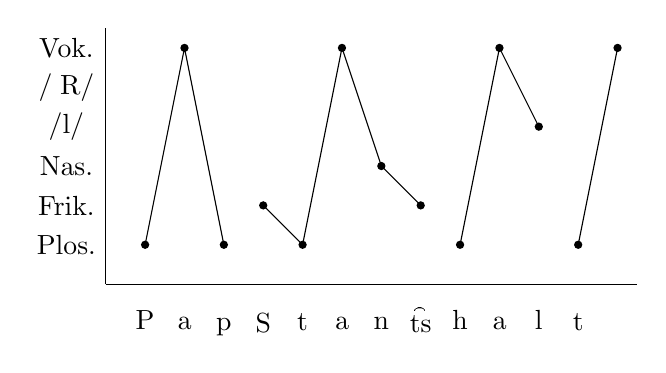
\begin{tikzpicture}[scale=0.5]
\draw[black] (-1,0) -- (12.5,0) ; % x axis
\draw[black] (-1,0) -- (-1,6.5); % y axis
\node at (-2,1) {Plos.};
\node at (-2,2) {Frik.};
\node at (-2,3) {Nas.};
\node at (-2,4) {\textipa{/l/}};
\node at (-2,5) {\textipa{/\;R/}};
\node at (-2,6) {Vok.};
\draw[black] (0,1)--(1,6)--(2,1);
\draw[black](3,2)--(4,1)--(5,6)--(6,3)--(7,2);
\draw[black](8,1)--(9,6)--(10,4);
\draw[black](11,1)--(12,6);
\fill (0,1) circle [radius=3pt];
\fill (1,6) circle [radius=3pt];
\fill (2,1) circle [radius=3pt];
\fill (3,2) circle [radius=3pt];
\fill (4,1) circle [radius=3pt];
\fill (5,6) circle [radius=3pt];
\fill (6,3) circle [radius=3pt];
\fill (7,2) circle [radius=3pt];
\fill (8,1) circle [radius=3pt];
\fill (9,6) circle [radius=3pt];
\fill (10,4) circle [radius=3pt];
\fill (11,1) circle [radius=3pt];
\fill (12,6) circle [radius=3pt];
\node at (0,-0.91){\textipa{P}};
\node at (1,-1){\textipa{a}};
\node at (2,-1.09){\textipa{p}};
\node at (3,-1){\textipa{S}};
\node at (4,-0.95){\textipa{t}};
\node at (5,-1){\textipa{a}};
\node at (6,-1){\textipa{n}};
\node at (7,-0.91){\textipa{\t{ts}}};
\node at (8,-0.91){\textipa{h}};
\node at (9,-1){\textipa{a}};
\node at (10,-0.91){\textipa{l}};
\node at (11,-0.95){\textipa{t}};
\node at (12,-1){\textipa{\textturna}};
\end{tikzpicture}}
\end{figure}
\end{minipage}


\end{frame}

}%% END LOESUNG	
%%%%%%%%%%%%%%%%%%%%%%%%%%%%%%%%%%%



%%%%%%%%%%%%%%%%%%%%%%%%%%%%%%%%%%
\subsection{Silbifizierung}

%% MyP: Contents
\iftoggle{sectoc}{
	\frame{
		%\begin{multicols}{2}
		\frametitle{~}
		\tableofcontents[currentsubsection, subsubsectionstyle=hide]
		%\end{multicols}
	}
}

%% StM: Contents
\iftoggle{gliederung}{
	
	\outline{
		\begin{itemize}
			
			\item Silbenmodelle
			%% CV-Modell
			%% Konstituentenmodell
			\item Silbengelenk
			\item \blaubf{Silbifizierung}
			\item Exkurs: Akzent
			\item Hausaufgabe
			
		\end{itemize}
	}
}
%%%%%%%%%%%%%%%%%%%%%%%%%%%%%%%%%%

\begin{frame}
\frametitle{Silbifizierung}

\begin{block}{Silbifizierung (auch Syllabierung)}
	Wörter in Silben einteilen
\end{block}

\begin{itemize}
	\item Wie würden Sie folgende Lautsequenzen silbifizieren?
	
	\ea ata, odo, eke
	\z
	
	\pause
	
	\item Ein einziger intervokalischer Konsonant wird immer als Silbenanlaut silbifiziert (universelles Prinzip: \textbf{Onset-Maximierung})


\end{itemize}

\begin{block}{Onsetmaximierung}
Bilde zuerst den größtmöglichen Silbenanlaut;\\
dann bilde den Silbenauslaut \citep[218]{Hall00a}
\end{block}

\end{frame}


%%%%%%%%%%%%%%%%%%%%%%%%%%%%%%%%%%
\begin{frame}
\frametitle{Onset-Maximierung}

\begin{block}{Onset-Maximierung}
Bilde zuerst den größtmöglichen Silbenanlaut;\\
dann bilde den Silbenauslaut \citep[218]{Hall00a}.
\end{block}


\begin{itemize}
\item Onset-Maximierung herleitbar aus:
\begin{enumerate}
\item Silbenanlautgesetz (CV häufiger als V), und
\item Silbenauslautgesetz (CVC$^{n} >$ CVC$^{n+1}$, wobei $n \geq 0$)
\end{enumerate}

\pause
\item Silbifizierung nicht über Morphemgrenzen hinweg! 
\item Ausnahme: Suffixe mit vokalischem Onset:

\ea
kind\#isch: \textipa{[kIn.dIS]}
\z

\ea
kind\#lich: \textipa{[kInt.lI\c{c}]}
\z

\item \# := Morphemgrenze

% Wenn man Morphmgrenzenbedingung weglassen würde, ergäbe sich Bra. ndschutz

% rek.nen vs. re.gnen

\end{itemize}

\end{frame}

%%%%%%%%%%%%%%%%%%%%%%%%%%%%%%%%%%%
\iftoggle{uebung}{
%%%%%%%%%%%%%%%%%%%%%%%%%%%%%%%%%%
%%%%%%%%%%%%%%%%%%%%%%%%%%%%%%%%%%
%\subsection{Übung}
%
%%% MyP: Contents
%\iftoggle{sectoc}{
%	\frame{
%		%\begin{multicols}{2}
%		\frametitle{~}
%		\tableofcontents[currentsubsection, subsubsectionstyle=hide]
%		%\end{multicols}
%	}
%}
%%%%%%%%%%%%%%%%%%%%%%%%%%%%%%%%%%

\begin{frame}
\frametitle{Übung}

\begin{itemize}
	\item Was bedeutet die Annahme des Sonoritätsprinzips und der Onset-Maximierung für die folgenden Beispielwörter:
	
	\ea
	Fabrik, Imker, neblig, Falter, regnen
	\z
	
	\item Welche Prinzipien bzw. Regularitäten werden verletzt bei:
\end{itemize}

\begin{minipage}{.3\textwidth}
\eal
\ex \textipa{[PE.b@]}
\ex \textipa{[PEb.@]}
\ex \textipa{[PEp.@]}
\ex \textipa{[PEp.b@]}
\zl
\end{minipage}


\end{frame}
%%%%%%%%%%%%%%%%%%%%%%%%

\begin{frame}
\frametitle{Übung}

\begin{itemize}
	\item Silbifizieren Sie folgende Segmentsequenzen \textbf{in zwei Schritten}
	\begin{itemize}
		\item Onsetmaximierungsprinzip
		\item Sonoritätsprinzip
	\end{itemize}
	
	\item Stellen Sie fest, ob alle Silben wohlgeformt sind.\\
	Falls nicht, benennen Sie die Verletzungen
	
	\ea
	\textipa{[o:tlIN5mSplag\textscr e:hOn]}
	\z
	
	% Otlingamsplagrehon
	\ea
	Blumentopferde
	\z
	
\end{itemize}

% blu.men.to.pfer.de

%\ea
%Urinstinkt
%\z	

\end{frame}


%%%%%%%%%%%%%%%%%%%%%%%%%%%%%%%%%%%%%%%

} 
%% END true = Q
%% BEGIN false = Q + A
{
%%%%%%%%%%%%%%%%%%%%%%%%%%%%%%%%%%
%\subsection{Übung}
%
%%% MyP: Contents
%\iftoggle{sectoc}{
%	\frame{
%		%\begin{multicols}{2}
%		\frametitle{~}
%		\tableofcontents[currentsubsection, subsubsectionstyle=hide]
%		%\end{multicols}
%	}
%}
%%%%%%%%%%%%%%%%%%%%%%%%%%%%%%%%%%

\begin{frame}
\frametitle{Übung}

\begin{itemize}
	\item Was bedeutet die Annahme des Sonoritätsprinzips und der Onset-Maximierung für die folgenden Beispielwörter:
	

	\ea Fabrik, Imker, neblig, Falter, regnen
	\z

\pause

	\begin{itemize}
	\item[] \textcolor{red}{\textipa{[fa:.b\textscr Ik]}, \pause
		\textipa{[PIm.k5]}, \pause
		\textipa{[ne:.blI\c{c}]}, \pause
		\textipa{[fal.t5]}, \pause
		\textipa{[\textscr e:.gn@n]}} \pause
	\item [] \textcolor{red}{Koda: *Obstruent vor Sonorant} 
	\item [] \textcolor{red}{Onset: *Sonorant vor Obstruent}
	\end{itemize}
	\pause
	\item Onset-Maximierung ist nicht strikt. Alternativ ginge auch \textipa{[ne:p.lI\c{c}]}, \textipa{[\textscr e:k.n@n]}.
	

	\item Welche Prinzipien bzw. Regularitäten werden verletzt bei:

%\begin{multicols}{2}
\begin{columns}
	\column{.25\textwidth}
	\eal
		\ex \textipa{[PE.b@]}
		\ex \textipa{[PEb.@]}
		\ex \textipa{[PEp.@]}
		\ex \textipa{[PEp.b@]}
	\zl

\column{.65\textwidth}
\pause

\begin{itemize}
	\item[] \textcolor{red}{\ras Kurzvokal} Lösung \zb Silbengelenk \textipa{[PE\.b@]}
	\item[] \textcolor{red}{\ras Auslautverhärtung}
	\item[] \textcolor{red}{\ras Onset-Maximierung}
	\item[] \textcolor{red}{\ras keine Regelverletzung}
\end{itemize}
	
%\end{multicols}
\end{columns}
\end{itemize}

\end{frame}

%%%%%%%%%%%%%%%%%%%%%%%%%%%%%%%%%%



\begin{frame}
\frametitle{Übung}

\begin{itemize}
\item Silbifizieren Sie folgende Segmentsequenzen \textbf{in zwei Schritten}
\begin{itemize}
	\item Onsetmaximierungsprinzip
	\item Sonoritätsprinzip
\end{itemize}

\item Stellen Sie fest, ob alle Silben wohlgeformt sind.\\
Falls nicht, benennen Sie die Verletzungen

\ea
\textipa{[o:tlIN5mSplag\textscr e:hOn]}\\ \pause
\alertred{zuerst Onset"=Maximierung: \textipa{o: . tlI . \ng {\textturna} . mSpla . g\textscr e: . hOn}\\
dann Anwendung des Sonoritätsprinzips: \textipa{o: . tlI\. \ng \textturna mS . pla . g\textscr e: . hOn}}


% Otlingamsplagrehon

\ex
Blumentopferde\\ \pause
\alertred{
	zuerst Onset-Maximierung: \textipa{blu: . m@ . ntO . pfE . {\textscr}d@}\\
dann Awendung des Sonoritätsprinzips: \textipa{blu: . m@n . tO . pfE{\textscr} . d@}
}
\z

\end{itemize}

% blu.men.to.pfer.de

%\ea
%Urinstinkt
%\z	

\end{frame}


% ' Stahl , tische     Hauptbetonung auf Stahl, Nebenbetonung auf Tische


}%% END LOESUNG	
%%%%%%%%%%%%%%%%%%%%%%%%%%%%%%%%%%%
%%%%%%%%%%%%%%%%%%%%%%%%%%%%%%%%%


%%%%%%%%%%%%%%%%%%%%%%%%%%%%%%%%%%
\subsection{Exkurs: Akzent}

%% MyP: Contents
\iftoggle{sectoc}{
	\frame{
		%\begin{multicols}{2}
		\frametitle{~}
		\tableofcontents[currentsubsection, subsubsectionstyle=hide]
		%\end{multicols}
	}
}

%% StM: Contents
\iftoggle{gliederung}{
	
	\outline{
		\begin{itemize}
			
			\item Silbenmodelle
			%% CV-Modell
			%% Konstituentenmodell
			\item Silbengelenk
			\item Silbifizierung
			\item \blaubf{Exkurs: Akzent}
			\item Hausaufgabe
			
		\end{itemize}
	}
}
%%%%%%%%%%%%%%%%%%%%%%%%%%%%%%%%%%

\begin{frame}
\frametitle{Exkurs: Akzent}

\begin{itemize}
\item Silben können \textbf{betont} oder \textbf{unbetont} sein, d.\,h. sie können einen Akzent tragen oder nicht
\item[]

\begin{block}{Akzent}
\textbf{Auditiver Eindruck der Prominenz eines Vokals} gegenüber einem anderen durch (relational, nicht absolut!):
\begin{itemize}
\item Lautstärke
\item Dauer
\item Höhere Tonlage
\item Ausgeprägtere Artikulationsbewegungen
\end{itemize}
\end{block}	 

\item[]
\item Man unterscheidet zwischen \textbf{Wort-} und \textbf{Satzakzent} (engl. \emph{stress} und \emph{accent})

\end{itemize}

\end{frame}



%%%%%%%%%%%%%%%%%%%%%%%%%%%%%%%%%%%
%%%%%%%%%%%%%%%%%%%%%%%%%%%%%%%%%%
%\subsubsection{Exkurs: Wortakzent}
%\frame{
%\begin{multicols}{2}
%\frametitle{~}
%	\tableofcontents[currentsection]
%\end{multicols}
%}
%%%%%%%%%%%%%%%%%%%%%%%%%%%%%%%%%%

\begin{frame}
\frametitle{Exkurs: Wortakzent}

\begin{itemize}
\item Was scheint die häufigste Betonung im Deutschen zu sein?

\ea
Mutter, Männer, Autos, Hühner, Lehrer, Kinder, alle \ldots
\z

\pause
\textbf{betont-unbetont (Trochäus)}

\item Ausnahmen (die je nach Theorie verschieden erklärt werden):

\end{itemize}

\begin{minipage}{.4\textwidth}

\eal 
\ex \textipa{['f\textscr aU]}
\ex \textipa{[mu.'zi:k]}
\ex \textipa{['le:.b@n.d@]}
\ex \textipa{[pa.pa.'g\t{aɪ}]}
\ex \textipa{[f\t{ɛɐ}.'Pa\textscr .b\t{aɪ}.t@n]}
\zl

\end{minipage}
\begin{minipage}{.5\textwidth}

%	\iftoggle{loesung}{
\begin{itemize}
\item[] \textcolor{red}{\ras nur eine Silbe }
\item[] \textcolor{red}{\ras Fremdwort}
\item [] \textcolor{red}{\ras Flektierte Elemente \ab{-de}}
\item [] \textcolor{red}{\ras Fremdwort}
\item [] \textcolor{red}{\ras Derivation \ab{ver-}}
\end{itemize}
%}

\end{minipage}

\end{frame}



%%%%%%%%%%%%%%%%%%%%%%%%%%%%%%%%%%%
%%%%%%%%%%%%%%%%%%%%%%%%%%%%%%%%%%
%\subsubsection{Exkurs: Satzakzent}
%\frame{
%\begin{multicols}{2}
%\frametitle{~}
%	\tableofcontents[currentsection]
%\end{multicols}
%}
%%%%%%%%%%%%%%%%%%%%%%%%%%%%%%%%%%

\begin{frame}
\frametitle{Exkurs: Satzakzent}

\begin{itemize}
\item In einem Satz können betonte Silben \textbf{noch weiter hervorgehoben} werden (dabei meist durch die Tonhöhe):

\eal 
\ex Géstern hat BAyern gewónnen.
\ex GÉStern hat Báyern gewónnen.
\ex Géstern hat Báyern geWONnen.
\zl
\item Die prominenteste Silbe im Satz wird meist mit \textbf{Großbuchstaben} dargestellt, sie trägt den Satzakzent

\item Durch diese Akzentuierung wird das gesamte Wort
hervorgehoben \ras\\ \textbf{Fokus des Satzes} (\gqq{Informationsstruktur})

\end{itemize}

\end{frame}



%%%%%%%%%%%%%%%%%%%%%%%%%%%%%%%%%%%
%%%%%%%%%%%%%%%%%%%%%%%%%%%%%%%%%%
%\subsubsection{Exkurs: Intonation}
%\frame{
%\begin{multicols}{2}
%\frametitle{~}
%	\tableofcontents[currentsection]
%\end{multicols}
%}
%%%%%%%%%%%%%%%%%%%%%%%%%%%%%%%%%%

\begin{frame}
\frametitle{Exkurs: Intonation}

\begin{block}{Intonation}
Tonhöhenverlauf (\gqq{Melodie}) einer Äußerung
\end{block}

\begin{itemize}
\item \textbf{Satztypen} können mittels Intonation unterschieden werden.

\item Sprechen Sie die folgenden Äußerungen mit fallender und steigender Intonation
\eal 
\ex Heute gewinnen die Bayern.
\ex Schon Schluss.
\zl
\pause
\textbf{Aussage-} \vs \textbf{Interrogativsatz}	

\end{itemize}

\end{frame}



%%%%%%%%%%%%%%%%%%%%%%%%%%%%%%%%%%

\begin{frame}
\frametitle{Disambiguierung}

Ambige ($\approx$ mehrdeutige) Sätze können mittels Intonation \gs{durch die sog. Hutkontur} \textbf{disambiguiert} werden: 

\begin{exe}
\ex  \label{exe:nicht}Alle Studenten haben die Klausur nicht bestanden.

	\begin{xlist}
	\ex Es ist nicht der Fall, dass alle Studenten die Klausur bestanden haben. \hfill $\lsem \neg \forall \rsem$
	\ex Für alle Studenten gilt, dass sie die Klausur nicht bestanden haben. \hfill $\lsem \forall \neg \rsem$
	\end{xlist}

\pause 

\ex /ALle Studenten haben die Klausur  NICHT\textbackslash\ bestanden.
\exr{exe:nicht}
	\begin{xlist}
	\ex Es ist nicht der Fall, dass alle Studenten die Klausur bestanden haben. \hfill $\lsem \neg \forall \rsem$
	\end{xlist}
\end{exe}


\end{frame}

%%%%%%%%%%%%%%%%%%%%%%%%%%%%%%%%%%
%%%%%%%%%%%%%%%%%%%%%%%%%%%%%%%%%%

\iftoggle{hausaufgabe}{

\subsection{Hausaufgabe}

%%% MyP: Contents
%\iftoggle{sectoc}{
%	\frame{
%		%\begin{multicols}{2}
%		\frametitle{~}
%		\tableofcontents[currentsubsection, subsubsectionstyle=hide]
%		%\end{multicols}
%	}
%}

%%% StM: Contents
%\iftoggle{gliederung}{
%	
%	\outline{
%		\begin{itemize}
%			
%			\item Silbenmodelle
%			%% CV-Modell
%			%% Konstituentenmodell
%			\item Silbengelenk
%			\item Silbifizierung
%			\item Exkurs: Akzent
%			\item \blaubf{Hausaufgabe}
%			
%		\end{itemize}
%	}
%}

%%%%%%%%%%%%%%%%%%%%%%%%%%%%%%%%%%
\begin{frame}%[allowframebreaks]
\frametitle{Hausaufgabe}
\begin{itemize}

\item[1.] Geben Sie eine \textbf{phonetische Transkription} der folgenden Wörter nach der \gqq{Standardaussprache} an, zeichnen Sie dabei die \textbf{Silbenstruktur} nach dem \textbf{Konstituentenmodell} und mit der \textbf{Skelettschicht} und geben Sie die \textbf{Sonoritätsprofile} an.

\eal\label{ex:HA1}
\ex Stimmenfang \label{ex:HA1a}
\ex Mittagessen\label{ex:HA1b}
\ex Bierdeckel\label{ex:HA1c}
\zl
\end{itemize}

\begin{block}{Sonoritätshierarchie (Zur Erinnerung)}
Vokal $>$ \textipa{/\textscr /} $>$ \textipa{/l/} $>$ Nasal $>$ Frikativ $>$ Plosiv \\
$x > y :=$ $x$ ist sonorer als $y$
\end{block}

\end{frame}

%%%%%%%%%%%%%%%%%%%%%%%%%%%%%%%%%%%%%%%%%%%%%%%%%%%%%

\begin{frame}
\begin{itemize}
\item[2.] Silbifizieren Sie folgende Segmentsequenzen \textbf{in zwei Schritten}:
\begin{itemize}
\item Onsetmaximierungsprinzip
\item Sonoritätsprinzip
\end{itemize}

Stellen Sie fest, ob alle Silben wohlgeformt sind. Falls nicht, benennen Sie die Verletzungen	
\ea\label{ex:HA2}
Urinstinkt
\z	
\item[3.] Geben Sie die standarddeutsche \textbf{phonetische Transkription} des Wortes \ab{Stahltische} inklusive der \textbf{Silbenstruktur} (mit X-Skelettschicht) an. Ermitteln Sie die \textbf{Kriterien}, die bei der Silbifizierung wirken.

\item[4.] Geben Sie die Gründe an, warum die folgenden Wörter aus phonetisch/""phonologischen Gründen im Deutschen nicht möglich sind:

\eal\label{ex:HA3}
\ex[*]{\textipa{['Napl.O:t]}}
\ex[*]{\textipa{[a\;R.'tUng]}}
\zl

\end{itemize}

\end{frame}

%%%%%%%%%%%%%%%%%%%%%%%%%%%%%%%%%%%

} 
%% END true = Q
%% BEGIN false = Q + A
{
%%%%%%%%%%%%%%%%%%%%%%%%%%%%%%%%%%

\subsection{Hausaufgabe}

%%% MyP: Contents
%\iftoggle{sectoc}{
%	\frame{
%		%\begin{multicols}{2}
%		\frametitle{~}
%		\tableofcontents[currentsubsection, subsubsectionstyle=hide]
%		%\end{multicols}
%	}
%}

%%% StM: Contents
%\iftoggle{gliederung}{
%	
%	\outline{
%		\begin{itemize}
%			
%			\item Silbenmodelle
%			%% CV-Modell
%			%% Konstituentenmodell
%			\item Silbengelenk
%			\item Silbifizierung
%			\item Exkurs: Akzent
%			\item \blaubf{Hausaufgabe}
%			
%		\end{itemize}
%	}
%}

%%%%%%%%%%%%%%%%%%%%%%%%%%%%%%%%%%
\begin{frame}%[allowframebreaks]
\frametitle{Hausaufgabe}
\begin{itemize}
	
	\item[1.] Geben Sie eine \textbf{phonetische Transkription} der folgenden Wörter nach der \gqq{Standardaussprache} an, zeichnen Sie dabei die \textbf{Silbenstruktur} nach dem \textbf{Konstituentenmodell} und mit der \textbf{Skelettschicht} und geben Sie die \textbf{Sonoritätsprofile} an.
	
	\eal\label{ex:HA1}
	\ex Stimmenfang \label{ex:HA1a}
	\ex Mittagessen\label{ex:HA1b}
	\ex Bierdeckel\label{ex:HA1c}
	\zl
\end{itemize}

\begin{block}{Sonoritätshierarchie (Zur Erinnerung)}
	Vokal $>$ \textipa{/\textscr /} $>$ \textipa{/l/} $>$ Nasal $>$ Frikativ $>$ Plosiv \\
	$x > y :=$ $x$ ist sonorer als $y$
\end{block}

\end{frame}

%%%%%%%%%%%%%%%%%%%%%%%%%%%%%%%%%%%%%%%%%%%%%%%%%%%%%

\begin{frame}
\begin{itemize}
\item[2.] Silbifizieren Sie folgende Segmentsequenzen \textbf{in zwei Schritten}:
\begin{itemize}
	\item Onsetmaximierungsprinzip
	\item Sonoritätsprinzip
\end{itemize}

Stellen Sie fest, ob alle Silben wohlgeformt sind.\\
Falls nicht, benennen Sie die Verletzungen.
\ea\label{ex:HA2}
Urinstinkt
\z	
\item[3.] Geben Sie die standarddeutsche \textbf{phonetische Transkription} des Wortes \ab{Stahltische} inklusive der \textbf{Silbenstruktur} (mit X-Skelettschicht) an. Ermitteln Sie die \textbf{Kriterien}, die bei der Silbifizierung wirken.

\item[4.] Geben Sie die Gründe an, warum die folgenden Wörter aus phonetisch/""phonologischen Gründen im Deutschen nicht möglich sind:

\eal\label{ex:HA3}
\ex[*]{\textipa{['Napl.O:t]}}
\ex[*]{\textipa{[a\;R.'tUng]}}
\zl

\end{itemize}

\end{frame}

%%%%%%%%%%%%%%%%%%%%%%%%%%%%%%%%%%%
}%% END hausaufgabe

\iftoggle{ha-loesung}{

\subsection*{Lösung Hausaufgabe}
%
%%% MyP: Contents
%\iftoggle{sectoc}{
%	\frame{
%		%\begin{multicols}{2}
%		\frametitle{~}
%		\tableofcontents[currentsubsection, subsubsectionstyle=hide]
%		%\end{multicols}
%	}
%}


%%%%%%%%%%%%%%%%%%%%%%%%%%%%%%%%%%
\begin{frame}%[allowframebreaks]
\frametitle{Lösung}
\begin{itemize}

\item[1.] Geben Sie eine \textbf{phonetische Transkription} der folgenden Wörter nach der \gqq{Standardaussprache} an, zeichnen Sie dabei die \textbf{Silbestruktur} nach dem \textbf{Konstituentenmodell} und mit der \textbf{Skelettschicht} und geben Sie die \textbf{Sonoritätsprofile} an.

\begin{exe}
\exi{(\ref{ex:HA1})}
\begin{xlist}
\ex Stimmenfang
\ex Mittagessen
\ex Bierdeckel
\end{xlist}
\end{exe}

\begin{block}{Sonoritätshierarchie (Zur Erinnerung)}
Vokal $>$ \textipa{/\textscr /} $>$ \textipa{/l/} $>$ Nasal $>$ Frikativ $>$ Plosiv \\
$x > y :=$ $x$ ist sonorer als $y$
\end{block}

\end{itemize}
\end{frame}

\begin{frame}

%\begin{minipage}{.35\textwidth}
%%%%%%%%%%%%%%
%%% Forestset Syllables

\newbox\foreststrutbox
\setbox\foreststrutbox=\hbox to 0pt{\phantom{\forestOve{standard node}{content}}}
\def\foreststrut{\copy\foreststrutbox}
\forestset{
GP1/.style 2 args={
for n={1}{baseline},
s sep=0pt, l sep=0pt,
for descendants={
l sep=0pt, l={#1},
anchor=base,calign=first,child anchor=north,
inner xsep=1pt,inner ysep=2pt,outer sep=0pt,s sep=0pt,
},
delay={
if content={}{phantom}{for children={no edge}},
for tree={
if content={O}{tier=OR}{},
if content={R}{tier=OR}{},
if content={N}{tier=N}{},
if content={x}{
tier=x,content={$\times$},outer xsep={#2},
for tree={calign=center},
for descendants={content format={\foreststrut\forestoption{content}}},
before drawing tree={outer xsep=0pt,delay={typeset node}},
s sep=4pt
}{},
},
},
before drawing tree={where content={}{parent anchor=center,child anchor=center}{}},
},
GP1/.default={5ex}{8.0pt},
associate/.style={%
tikz+={\draw(!)--(!#1);}},
spread/.style={
before drawing tree={tikz+={\draw[dotted](!)--(!#1);}}},
govern/.style={
before drawing tree={tikz+={\draw[->](!)--(!#1);}}},
p-govern/.style={
before drawing tree={tikz+={\draw[->](.north) to[out=150,in=30] (!#1.north);}}},
no p-govern/.style={
before drawing tree={tikz+={\draw[->,loosely dashed](.north) to[out=150,in=30] (!#1.north);}}},
encircle/.style={before drawing tree={circle,draw,inner sep=0pt}},
fen/.style={pin={[font=\footnotesize,inner sep=1pt,pin edge=<-]10:\textsc{Fen}}},
el/.style={content=\textsc{\textbf{##1}}},
head/.style={content=\textsc{\textbf{\underline{##1}}}},
llap/.style={
tikz+={%
\edef\forest@temp{\noexpand\node[\option{node options},
anchor=base east,at=(.base east)]}%
\forest@temp{#1\phantom{\option{environment}}};
}
},
rlap/.style={
tikz+={%
\edef\forest@temp{\noexpand\node[\option{node options},
anchor=base west,at=(.base west)]}%
\forest@temp{\phantom{\option{environment}}#1};
}
},
}
%%%%%%%%%%%%%

\begin{minipage}{.2\textwidth}
\centering
Zu (\ref{ex:HA1a}):
\end{minipage}
%
\begin{minipage}{.7\textwidth}
\begin{figure}
\footnotesize
\centering
\begin{forest} MyP edges, [, phantom
[$\sigma$
[O [x, tier=word [\textipa{S}]] [x, tier=word [\textipa{t}]]]
[R [N [x, tier=word [\textipa{I}]]] [K [x, name=x [\textipa{m}]]]]
]
[$\sigma$
[O, name=onset]
[R [N [x [\textipa{@}]]] [K [x [\textipa{n}]]]]
]
[$\sigma$
[O [x, tier=word [\textipa{f}]]]
[R [N [x [\textipa{a}]]] [K [x [\textipa{N}]]]]
]
]				
{
\draw[black] (x.north)--(onset.south);
}
\end{forest}

\pause

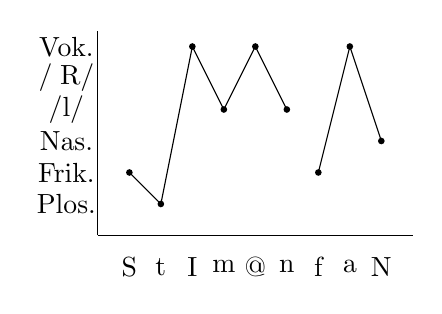
\begin{tikzpicture}[scale=0.4]
\draw[black] (-1,0) -- (9,0) ; % x axis
\draw[black] (-1,0) -- (-1,6.5); % y axis
\node at (-2,1) {Plos.};
\node at (-2,2) {Frik.};
\node at (-2,3) {Nas.};
\node at (-2,4) {\textipa{/l/}};
\node at (-2,5) {\textipa{/\;R/}};
\node at (-2,6) {Vok.};
\draw[black] (0,2) -- (1,1) -- (2,6) -- (3,4) -- (4,6) -- (5,4);
\draw[black] (6,2) -- (7,6) -- (8,3);
\node at (0,-1) {\textipa{S}};
\node at (1,-1) {\textipa{t}};
\node at (2,-1) {\textipa{I}};
\node at (3,-1) {\textipa{m}};
\node at (4,-1) {\textipa{@}};
\node at (5,-1) {\textipa{n}};
\node at (6,-1) {\textipa{f}};
\node at (7,-1) {\textipa{a}};
\node at (8,-1) {\textipa{N}};
\fill (0,2) circle [radius=3pt];
\fill (1,1) circle [radius=3pt];
\fill (2,6) circle [radius=3pt];
\fill (3,4) circle [radius=3pt];
\fill (4,6) circle [radius=3pt];
\fill (5,4) circle [radius=3pt];
\fill (6,2) circle [radius=3pt];
\fill (7,6) circle [radius=3pt];
\fill (8,3) circle [radius=3pt];
\end{tikzpicture}
\end{figure}

\end{minipage}
\end{frame}

%%%%%%%%%%%%%%%%%%%%%%%%%%%%%%%%%%%%%%%%%%%%%%%

\begin{frame}		

\begin{minipage}{.2\textwidth}
\centering
Zu (\ref{ex:HA1b})
\end{minipage}	
\begin{minipage}{.7\textwidth}
\footnotesize
\centering
\begin{forest} MyP edges, [, phantom
[$\sigma$
[O [x, tier=word [\textipa{m}]]] 
[R [N [x, tier=word [\textipa{I}]]] [K [x, name=x1 [\textipa{t}]]]]
]
[$\sigma$
[O, name=onset1]
[R [N [x [\textipa{a:}, name=a]]
[x, name=ax]] [K [x [\textipa{k}]]]]
]
[$\sigma$
[O [x, tier=word [\textipa{P}]]]
[R [N [x [\textipa{E}]]] [K [x, name=x2 [\textipa{s}]]]]
]
[$\sigma$
[O, name=onset2]
[R [N [x [\textipa{\textsyllabic{n}}]]]
]
]]
{
\draw[black] (x1.north)--(onset1.south);
\draw[black] (x2.north)--(onset2.south);
\draw[black] (a.north)--(ax.south);
}
\end{forest}

\pause

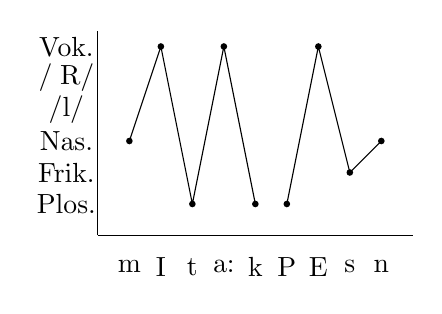
\begin{tikzpicture}[scale=0.4]
\draw[black] (-1,0) -- (9,0) ; % x axis
\draw[black] (-1,0) -- (-1,6.5); % y axis
\node at (-2,1) {Plos.};
\node at (-2,2) {Frik.};
\node at (-2,3) {Nas.};
\node at (-2,4) {\textipa{/l/}};
\node at (-2,5) {\textipa{/\;R/}};
\node at (-2,6) {Vok.};
\draw[black] (0,3) -- (1,6) -- (2,1) -- (3,6) -- (4,1);
\draw[black] (5,1) -- (6,6) -- (7,2) -- (8,3);
\node at (0,-1) {\textipa{m}};
\node at (1,-1) {\textipa{I}};
\node at (2,-1) {\textipa{t}};
\node at (3,-1) {\textipa{a:}};
\node at (4,-1) {\textipa{k}};
\node at (5,-1) {\textipa{P}};
\node at (6,-1) {\textipa{E}};
\node at (7,-1) {\textipa{s}};
\node at (8,-1) {\textipa{\textsyllabic{n}}};
\fill (0,3) circle [radius=3pt];
\fill (1,6) circle [radius=3pt];
\fill (2,1) circle [radius=3pt];
\fill (3,6) circle [radius=3pt];
\fill (4,1) circle [radius=3pt];
\fill (5,1) circle [radius=3pt];
\fill (6,6) circle [radius=3pt];
\fill (7,2) circle [radius=3pt];
\fill (8,3) circle [radius=3pt];
\end{tikzpicture}
\end{minipage}

\end{frame}

%%%%%%%%%%%%%%%%%%%%%%%%%%%%%%%%%%%%%%%%%%%%

\begin{frame}		

\begin{minipage}{.2\textwidth}
\centering
Zu (\ref{ex:HA1b})  (alternative Lösung):
\end{minipage}	
%\end{minipage}%
\begin{minipage}{.7\textwidth}
\footnotesize
\centering
\begin{forest} MyP edges, [, phantom
[$\sigma$
[O [x, tier=word [\textipa{m}]]] 
[R [N [x, tier=word [\textipa{I}]]] [K [x, name=x1 [\textipa{t}]]]]
]
[$\sigma$
[O, name=onset1]
[R [N [x [\textipa{a:}, name=a]]
[x, name=ax]] [K [x [\textipa{k}]]]]
]
[$\sigma$
[O [x, tier=word [\textipa{P}]]]
[R [N [x [\textipa{E}]]] [K [x, name=x2 [\textipa{s}]]]]
]
[$\sigma$
[O, name=onset2]
[R [N [x [\textipa{@}]]] [K [x [\textipa{n}]]]]
]
]
{
\draw[black] (x1.north)--(onset1.south);
\draw[black] (x2.north)--(onset2.south);
\draw[black] (a.north)--(ax.south);
}
\end{forest}

\pause

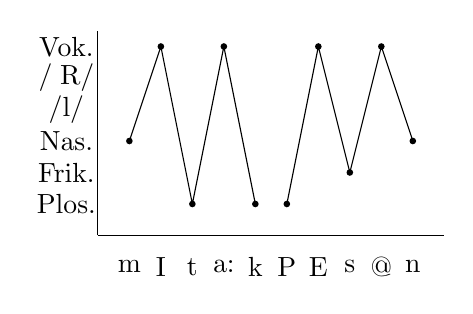
\begin{tikzpicture}[scale=0.4]
\draw[black] (-1,0) -- (10,0) ; % x axis
\draw[black] (-1,0) -- (-1,6.5); % y axis
\node at (-2,1) {Plos.};
\node at (-2,2) {Frik.};
\node at (-2,3) {Nas.};
\node at (-2,4) {\textipa{/l/}};
\node at (-2,5) {\textipa{/\;R/}};
\node at (-2,6) {Vok.};
\draw[black] (0,3) -- (1,6) -- (2,1) -- (3,6) -- (4,1);
\draw[black] (5,1) -- (6,6) -- (7,2) -- (8,6) -- (9,3);
\node at (0,-1) {\textipa{m}};
\node at (1,-1) {\textipa{I}};
\node at (2,-1) {\textipa{t}};
\node at (3,-1) {\textipa{a:}};
\node at (4,-1) {\textipa{k}};
\node at (5,-1) {\textipa{P}};
\node at (6,-1) {\textipa{E}};
\node at (7,-1) {\textipa{s}};
\node at (8,-1) {\textipa{@}};
\node at (9,-1) {\textipa{n}};
\fill (0,3) circle [radius=3pt];
\fill (1,6) circle [radius=3pt];
\fill (2,1) circle [radius=3pt];
\fill (3,6) circle [radius=3pt];
\fill (4,1) circle [radius=3pt];
\fill (5,1) circle [radius=3pt];
\fill (6,6) circle [radius=3pt];
\fill (7,2) circle [radius=3pt];
\fill (8,6) circle [radius=3pt];
\fill (9,3) circle [radius=3pt];
\end{tikzpicture}
\end{minipage}

\end{frame}


%%%%%%%%%%%%%%%%%%%%%%%%%%%%%%%%%%%%%%%%%%%%%%%

\begin{frame}

\begin{minipage}{.2\textwidth}
\centering
Zu (\ref{ex:HA1c}):
\end{minipage}	
\begin{minipage}{.7\textwidth}

\begin{figure}
\footnotesize
\centering
\begin{forest} MyP edges, [, phantom
[$\sigma$
[O [x,tier=word [\textipa{b}]]]
[R [N [x, tier=word [\textipa{i:}, name=i]] [x,name=x1]] [K [x [\textipa{5}]]]]
]
[$\sigma$
[O [x, tier=word [\textipa{d}]]]
[R [N [x [\textipa{E}]]] [K [x, name=x [\textipa{k}]]]]
]
[$\sigma$
[O, name=onset]
[R [N [x, tier=word [\textipa{@}]]] [K [x [\textipa{l}]]]]
]
]
{
\draw[black] (x1.south)--(i.north);
\draw[black] (x.north)--(onset.south);
}
\end{forest}

\pause

\scalebox{.85}{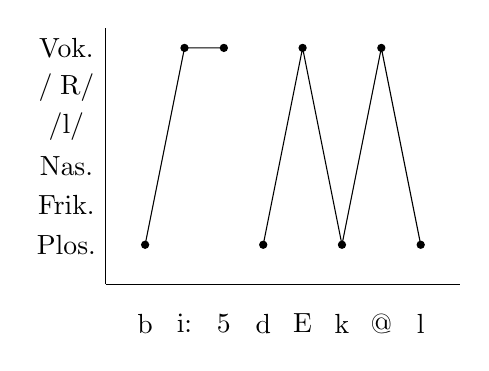
\begin{tikzpicture}[scale=0.5]
\draw[black] (-1,0) -- (8,0) ; % x axis
\draw[black] (-1,0) -- (-1,6.5); % y axis
\node at (-2,1) {Plos.};
\node at (-2,2) {Frik.};
\node at (-2,3) {Nas.};
\node at (-2,4) {\textipa{/l/}};
\node at (-2,5) {\textipa{/\;R/}};
\node at (-2,6) {Vok.};
\draw[black] (0,1) -- (1,6) -- (2,6);
\draw[black] (3,1) -- (4,6) -- (5,1) -- (6,6) -- (7,1);
\node at (0,-1) {\textipa{b}};
\node at (1,-1) {\textipa{i:}};
\node at (2,-1) {\textipa{5}};
\node at (3,-1) {\textipa{d}};
\node at (4,-1) {\textipa{E}};
\node at (5,-1) {\textipa{k}};
\node at (6,-1) {\textipa{@}};
\node at (7,-1) {\textipa{l}};
\fill (0,1) circle [radius=3pt];
\fill (1,6) circle [radius=3pt];
\fill (2,6) circle [radius=3pt];
\fill (3,1) circle [radius=3pt];
\fill (4,6) circle [radius=3pt];
\fill (5,1) circle [radius=3pt];
\fill (6,6) circle [radius=3pt];
\fill (7,1) circle [radius=3pt];
\end{tikzpicture}}
\end{figure}
\end{minipage}
%
%
\end{frame}
%%%%%%%%%%%%%%%%%%%%%%%%%%%%%%%%%%%%%%%%%%%%%%%%%%%

\begin{frame}
\begin{itemize}
\item[2.] Silbifizieren Sie folgende Segmentsequenzen \textbf{in zwei Schritten}:
\begin{itemize}
\item Onsetmaximierungsprinzip
\item Sonoritätsprinzip
\end{itemize}

Stellen Sie fest, ob alle Silben wohlgeformt sind.\\
Falls nicht, benennen Sie die Verletzungen.

\begin{exe}
\exr{ex:HA2} Urinstinkt
\pause
\begin{xlist}
\ex \textipa{[Pu.\;RI.nStInkt]} (Onsetmaximierung) \pause
\ex \textipa{[Pu.\;RIn.(\,S\,)tInkt]} (Sonoritätsprinzip, \textipa{S} ist extrasilbisch) \pause
\ex \textipa{[Pu5.PIn.stinkt]} (Silbifizierung)
\end{xlist}
\end{exe}
\pause
\item (\ref{ex:HA2}a) und (\ref{ex:HA2}b) sind einfach nach der Lautfolge silbifiziert.\\
Silbifizierung erfolgt jedoch auf der Ebene des phonologischen Wortes.\\
Daher werden die phonologischen Wörter \ab{ur-} und \ab{Instinkt} einzeln silbifiziert.
\end{itemize}
\end{frame}

%%%%%%%%%%%%%%%%%%%%%%%%%%%%%%%%%%%%%%%%%%%%%%%%

\begin{frame}
\begin{itemize}	
\item[3.] Geben Sie die standarddeutsche \textbf{phonetische Transkription} des Wortes \ab{Stahltische} inklusive der \textbf{Silbenstruktur} (mit X-Skelettschicht) an. Ermitteln Sie die \textbf{Kriterien}, die bei der Silbifizierung wirken.
\end{itemize}

\pause

\begin{minipage}{.5\textwidth}
\begin{figure}
\scalebox{.8}{\begin{forest}
MyP edges [, phantom
[$\sigma$
[O 
[x, tier=word[\textipa{S}]]
[x, tier=word[\textipa{t}]]
]
[R
[N
[x, tier=word[\textipa{a:}, name=a]]
[x, name=x]
]
[K[x[\textipa{l.}]]]
]
]
[$\sigma$
[O [x, tier=word[\textipa{t}]]]
[R
[N
[x[\textipa{I}]]
]
[K
[x,name=S[\textipa{S}] ]
]
]
]
[$\sigma$
[O, name=o]
[R
[N
[x[\textipa{@}]]
]
]
]
]
\draw[black](o.south)--(S.north);
\draw[black](a.north)--(x.south);
\end{forest}}
\end{figure}
\end{minipage}
\begin{minipage}{.45\textwidth}
	
\pause	
	
\begin{itemize}
\item Onset-Maximierung \pause
\item Sonoritätshierarchie im Onset: *Sonorant vor Obstruent (*[\textipa{lt}]) \pause
\item Silbengelenk nach ungespanntem, betonten Vokal
\end{itemize}
\end{minipage}

\end{frame}

%%%%%%%%%%%%%%%%%%%%%%%%%%%%%%%%%%%%%

\begin{frame}
\begin{itemize}

\item[4.] Geben Sie die Gründe an, warum die folgenden Wörter aus phonetisch/""phonologischen Gründen im Deutschen nicht möglich sind:

\begin{exe}
	\exr{ex:HA3}
	\begin{xlist}
		\ex[*]{ \textipa{['Napl.O:t]}
			\only<2->{: \textcolor{red}{Onset-Maximierung \textipa{[pl]}, \textipa{[N]} steht am Wortanfang, \textipa{[O]} ist ungespannt und lang}} }
		\ex[*]{ \textipa{[a\;R.'tUng]}
			\only<3->{: \textcolor{red}{Auslautverhärtung, regressive velare nasale Assimilation, Knacklaut}} }
\end{xlist}

\end{exe}

\end{itemize}

\end{frame}

}%% END LOESUNG	

%%%%%%%%%%%%%%%%%%%%%%%%%%%%%%%%%%%%
%%%%%%%%%%%%%%%%%%%%%%%%%%%%%%%%%%%

%%%%%%%%%%%%%%%%%%%%%%%%%%%%%%%%%%%



